\section{Lý thuyết về grasping}
Grasping \cite{prattichizzo2016grasping} hay nắm giữ, là một thành phần cốt lõi của thao tác robot, bởi vì nó cho phép robot kiểm soát hoàn toàn chuyển động của vật thể. Grasp có thể được hiểu là quá trình trong đó robot (thường là bàn tay robot, gripper, hoặc ngón kẹp) tạo và duy trì tiếp xúc với một vật thể nhằm kiểm soát lực - mô men tác dụng lên vật, giúp robot nhấc, giữ, thao tác hoặc di chuyển vật thể một cách ổn định. Phần này trình bày các khái niệm nền tảng của grasping, tập trung chủ yếu vào phần đẩy trên mặt phẳng (planar pushing) bao gồm mô hình tiếp xúc, biểu diễn wrench, Grasp Map, Grasp Wrench Space, force-closure và form-closure. Đây là nền tảng lý thuyết quan trọng để hiểu các bài toán nâng cao như thao tác tinh vi và đặc biệt là trong thao tác không cầm nắm (non-prehensile manipulation) như bài toán đa robot phối hợp đẩy vật, trong đó lực tương tác và cấu hình tiếp xúc đóng vai trò quyết định đến chuyển động của vật thể. Các lý thuyết được trình bày được tham khảo từ sách Handbook of Robotics bản 2008 \cite{sicilianoKhatib2008SHR} và slide bài giảng về Fundamentals of Grasping trong khóa học Principles of Robot Autonomy II của đại học Stanford.
\subsection{Các kiểu và mô hình tiếp xúc}
Mô hình tiếp xúc (contact model) là nền tảng trong phân tích và tổng hợp grasping, vì lực và mô men mà robot có thể tạo ra đều được truyền qua các điểm tiếp xúc giữa robot và vật thể. Việc lựa chọn mô hình tiếp xúc phù hợp có ảnh hưởng trực tiếp đến khả năng sinh không gian wrench, điều kiện force-closure, và toàn bộ quá trình đánh giá chất lượng grasp. Tiếp xúc có thể được chia thành ba kiểu cơ bản bao gồm tiếp xúc điểm, tiếp xúc đường và tiếp xúc mặt. Trong đó tiếp xúc điểm (Hình \ref{fig:contact_model}), đặc biệt là tiếp xúc điểm - mặt phẳng à kiểu tiếp xúc phổ biến, ổn định nhất và gần như luôn được sử dụng trong phân tích grasping vì các điểm tiếp xúc khả thi đối với hầu hết các vật thể gần như luôn là các điểm trên bề mặt phẳng chứ không phải các cạnh hoặc các điểm nhọn. Mục đích của mô hình tiếp xúc là xác định các lực và mô men có thể truyền qua điểm tiếp xúc đó.

\begin{figure}[H]
    \centering
    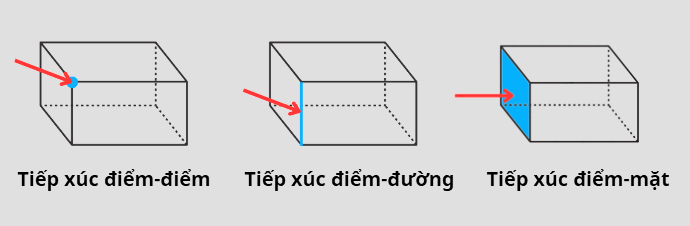
\includegraphics[scale=0.7]{chapter3/image/contact_type.png}
    \caption{Các kiểu tiếp xúc điểm}
    \label{fig:contact_model}
\end{figure}

Xét một hệ toạ độ cục bộ tại điểm tiếp xúc, với trục z trùng với pháp tuyến của bề mặt, chiều dương hướng vào trong vật. Khi đó, lực tác dụng tại tiếp xúc $\mathbf{f}$ có thể được phân tách thành hai thành phần: lực pháp tuyến và lực tiếp tuyến.
\begin{equation}
    \mathbf{f} = \mathbf{f}_{\mathrm{normal}} + \mathbf{f}_{\mathrm{tangent}}
\label{eq:f}
\end{equation}
trong đó $\mathbf{f}_{\mathrm{normal}} = [0,\, 0,\, f_z]^{T}$ là lực pháp tuyến với độ lớn là $f_z$,còn $\mathbf{f}_{\mathrm{tangent}} = [f_x,\, f_y,\, 0]^{T}$ là lực tiếp tuyến tại bề mặt.

\begin{figure}[H]
    \centering
    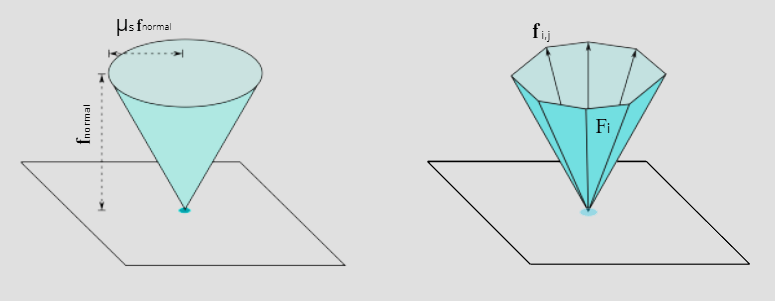
\includegraphics[scale=0.7]{chapter3/image/fricone.png}
    \caption{Nón ma sát đầy đủ(trái) và dạng xấp xỉ(phải)}
    \label{fig:fricone}
\end{figure}
Do đặc tính hình học, lực pháp tuyến phải có hướng ép vào vật ($f_z \geq 0$), còn lực tiếp tuyến nằm trên mặt phẳng tiếp xúc. Dựa trên mức độ tự do mà tiếp xúc có thể truyền, ba loại mô hình tiếp xúc thường được sử dụng, mỗi loại có một tập $\mathcal{F}$ các lực có thể được tác dụng vào tại điểm khác nhau bao gồm :

\begin{itemize}
    \item \textit{Tiếp xúc điểm không ma sát (Frictionless Point Contact)}: Tiếp xúc chỉ truyền được lực theo phương pháp tuyến và hoàn toàn không truyền lực tiếp tuyến hay mô men. Loại tiếp xúc này thường xuất hiện trong các phân tích form-closure, nơi không dựa vào ma sát để giữ vật. Tập lực cho phép đơn giản chỉ gồm:
    \begin{equation}
        \mathcal{F} = \{\, \mathbf{f}_{\mathrm{normal}} \mid f_z \geq 0 \,\}
    \label{eq:frlesscon}
    \end{equation}
    \item \textit{Tiếp xúc điểm có ma sát (Point Contact with Friction)}: Ở mô hình này, tiếp xúc có thể truyền lực theo cả phương tiếp tuyến, nhưng bị giới hạn bởi nón ma sát Coulomb như trong hình (\ref{fig:fricone}) bên trái với hệ số ma sát $\mu_s$, điều này đảm bảo lực tiếp tuyến không vượt quá khả năng chống trượt của tiếp xúc. Trong thực tế, để tính toán thuận tiện hơn, nón ma sát thường được thay bằng một đa diện xấp xỉ như hình (\ref{fig:fricone}) bên phải. Đây là loại tiếp xúc phổ biến nhất trong các kiểu nắm bắt force-closure. Tập lực cho phép:
    \begin{equation}
        \mathcal{F} = \{\, \mathbf{f} \mid \|\mathbf{f}_{\mathrm{tangent}}\| \leq \mu_s \|\mathbf{f}_{\mathrm{normal}}\|,\; f_z \geq 0 \,\}
    \label{eq:frcon}
    \end{equation}
    \item \textit{Tiếp xúc ngón tay mềm (Soft-Finger Contact)}: Ngoài lực pháp tuyến và lực tiếp tuyến, mô hình này cho phép truyền thêm một mô men xoắn quanh trục pháp tuyến tiếp xúc. Do đó, soft-finger có khả năng chống xoay tốt hơn, đặc biệt hữu ích trong các gripper dùng vật liệu mềm. Ràng buộc lực và mô men được mô tả bởi:
    \begin{equation}
        \mathcal{F} = \{\, (\mathbf{f}, \tau_{\mathrm{normal}}) \mid \|\mathbf{f}_{\mathrm{tangent}}\| \leq \mu_s \|\mathbf{f}_{\mathrm{normal}}\|,\;f_z \ge 0,\;|\tau_{\mathrm{normal}}| \le \gamma f_z\,\}
    \label{eq:softcon}
    \end{equation}
    trong đó hệ số $\gamma$ phản ánh khả năng truyền mô men của vật liệu tiếp xúc.
\end{itemize}

\subsection{Wrench}
Wrench là một đại lượng dạng vector mô tả lực và mô men đang tác dụng lên vật thể. Với một lực $\mathbf{f}\in \mathbb{R}^2$ và mô men $\boldsymbol{\tau}$ tác dụng lên vật tại khối tâm, wrench được viết trong một hệ quy chiếu gắn với vật thể dưới dạng vector ghép: 
\begin{equation}
    \mathbf{w} = [ \mathbf{f}, \,  \boldsymbol{\tau}]^{T} \in \mathbb{R}^3
\label{eq:wrench}
\end{equation}

Mỗi điểm tiếp xúc $i$ trong grasp tác dụng một wrench lên vật thể. Ngoài ra mô men $\boldsymbol{\tau_i}$ còn có thể tính bẳng công thức $\boldsymbol{\tau_i} = \mathbf{r}_i \times \mathbf{f}_i$ với $\mathbf{r}_i$ là cánh tay đòn tương ứng tại điểm tiếp xúc thứ $i$, khi đó ta có thể biểu diễn lại vector wrench dưới dạng:
\begin{equation}
    \mathbf{w}_i = [ \mathbf{f}_i, \,  \lambda (\mathbf{r}_i \times \mathbf{f}_i)]^{T},
\label{eq:wrench1}
\end{equation}
trong đó hằng số $\lambda \in \mathbb{R}$ có thể được chọn để điều chỉnh tỷ lệ của chiều mô men do tùy vào đơn vị đo mà chiều mô men có thể lớn hoặc bé hơn nhiều so với chiều về lực.

Dựa trên định nghĩa về wrench, grasp có thể được định nghĩa như tập các wrench khả thi có thể sinh ra từ tập điểm tiếp xúc của grasp đấy. Về mặt toán học, lực $\mathbf{f}_i$ tại điểm tiếp xúc thứ $i$ có thể được ánh xạ tuyến tính sang wrench $\mathbf{w}_i$ trên vật tương ứng bằng phép ánh xạ:
\begin{equation}
    \mathbf{w}_i = G_i \mathbf{f}_i
\label{eq:wrenchi}
\end{equation}
trong đó ma trận $G_i$ là một ma trận cơ sở wrench (wrench basis matrix) gồm phép biến đổi từ hệ toạ độ tại điểm tiếp xúc sang hệ toạ độ toàn cục của vật thể, ma trận tổng hợp $G = [G_1 \ldots G_k]$ được gọi là grasp map với k là số điểm tiếp xúc. Tổng wrench tác dụng lên vật từ toàn bộ k các tiếp xúc này là:
\begin{equation}
    \mathbf{w} = \sum_{i=1}^{k} G_i \mathbf{f}_i
\label{eq:wrench2}
\end{equation}

\subsection{Grasp Wrench Space}
Khi một mô hình tiếp xúc cụ thể đã được lựa chọn, một grasp có thể được phân tích bằng cách xem xét không gian grasp wrench space(GWS) $\mathcal{W}$. Không gian này là một tập con của không gian wrench, được định nghĩa là tập tất cả các wrench $\mathbf{w}$ có thể truyền lên vật thể thông qua các lực có khả thi. Không gian này thể hiện khả năng thao tác của grasp thông qua các wrench mà nó tạo ra, cụ thể với một grap với k điểm tiếp xúc ta có:

\begin{equation}
    \mathcal{W} = \left\{\mathbf{w} \;\middle|\;\mathbf{w} = \sum_{i=1}^{k} G_i \mathbf{f}_i,\;\mathbf{f}_i \in \mathcal{F}_i,\;i=1,\dots,k\right\}
\label{eq:gws}
\end{equation}

Nói cách khác, một grasp wrench space $\mathcal{W}$ có thể được xác định thông qua kết quả của phương trình (\ref{eq:wrench2}) khi xét tất cả với tổng hợp các lực khả thi có thể tác dụng  $\{\mathbf{f}_i\}_{i=1}^k$. Tuy nhiên trong thực tế, việc tính toán chính xác không gian này thường rất phức tạp và tốn chi phí tính toán. Do đó, người ta thường sử dụng cách tiếp cận thay thế để đặc trưng hoá một grasp là sử dụng grasp wrench hull, một đại lượng có thể được tính toán hiệu quả hơn. Wrench hull là một đối tượng hình học biểu diễn tập hợp tất cả các wrench khả thi được tạo ra bởi một hệ tiếp xúc, dưới dạng bao lồi của các wrench cơ sở, giả sử từ tập các tiếp xúc sinh ra các wrench rời rạc $w_\text{set} = [w_1 \ldots w_n]$, khi đó wrench hull được định nghĩa là:

\begin{equation}
    \widetilde{\mathcal{W}} = \left\{\sum_{i=1}^{N} \alpha_i \mathbf{w}_i \;\middle|\;\alpha_i \ge 0,\;\sum_{i=1}^{N} \alpha_i = 1\right\}
\label{eq:gwh}
\end{equation}

\subsection{Đánh giá grasp}

Nhìn chung nếu grasp wrench space càng lớn, grasp có thể chống lại được tập wrench lớn hơn đến từ môi trường, từ đó tạo ra một grasp vững hơn. Tuy nhiên để đánh giá một cách chi tiết, các tiêu chí cụ thể cần được nêu ra để xác định liệu một thao tác nắm giữ có “tốt” hay không, một trong số những tiêu chí cơ bản và phổ biến nhất là yếu tố closure, hay tính đóng kín. Grasp closure xảy ra khi cấu hình nắm giữ có thể chống đỡ được mọi nhiễu loạn bên ngoài tác động lên vật thể. Nói cách khác, đối với bất kỳ lực hay mô-men nào cố gắng làm vật thể rời khỏi tay robot, hệ các tiếp xúc phải có khả năng sinh ra một wrench đối kháng thích hợp để duy trì trạng thái nắm giữ. Ví dụ khi vật thể đang được đẩy bởi bầy robot bị va chạm với tường hay một vật thể khác, một grasp có closure sẽ vẫn duy trì được tiếp xúc giữa robot và vật chứ không để vật bị văng ra. Mặc dù trong thực tế rất khó có thể bảo đảm chống lại mọi nhiễu loạn có thể xuất hiện, khái niệm closure vẫn đặc biệt hữu ích để phân tích tính bền vững của một grasp. Grasp closure có thể được phân loại thành hai loại chính, bao gồm:
\begin{itemize}
    \item \textit{Form closure - đóng kín hình học}: Vật thể bị khóa hoàn toàn bởi cấu hình hình học của các tiếp xúc. Trong trạng thái này, vật không thể di chuyển theo bất kỳ phương nào mà không vi phạm ràng buộc hình học, nghĩa là ngay cả khi không có ma sát, vật vẫn bị “giam giữ” bởi cấu trúc kẹp. Do đó, form closure mang tính chất hình học thuần túy: các tiếp xúc được bố trí sao cho vật thể không còn đường thoát và không có độ rung lắc trong không gian cấu hình. Tuy nhiên, để đạt được form closure trong không gian 3D, số lượng tiếp xúc phải tương đối nhiều, ví dụ tối thiểu bảy tiếp điểm cho vật 3D, điều này khiến nó ít phổ biến trong các bộ kẹp robot thông thường.
    \item \textit{Force closure - đóng kín về lực}: Không yêu cầu khóa hình học tuyệt đối mà dựa vào khả năng sinh lực của các tiếp xúc có ma sát. Một grasp được xem là đạt force closure khi tập các lực và mô-men mà robot có thể tạo ra tại các điểm tiếp xúc đủ để chống lại mọi nhiễu loạn từ môi trường, về mặt hình học có thể hiểu đơn giản là gốc tọa độ trong không gian wrench nằm trong miền grasp wrench space, không được nằm trên cạnh hay mặt phẳng của GWS.Vì dựa trên ma sát, force closure thường yêu cầu ít điểm tiếp xúc hơn so với form closure, ví dụ ba điểm tiếp xúc với ma sát có thể tạo force closure trong 3D. Đồng thời, đây là dạng closure phản ánh đúng thực tế vận hành của robot, bởi phần lớn robot trong thực tế dựa vào ma sát để duy trì và điều khiển vật thể. Chính vì vậy, đánh giá force closure là trọng tâm trong hầu hết các nghiên cứu và ứng dụng liên quan đến chất lượng grasp trong robot học.
\end{itemize}

\begin{figure}[H]
    \centering
    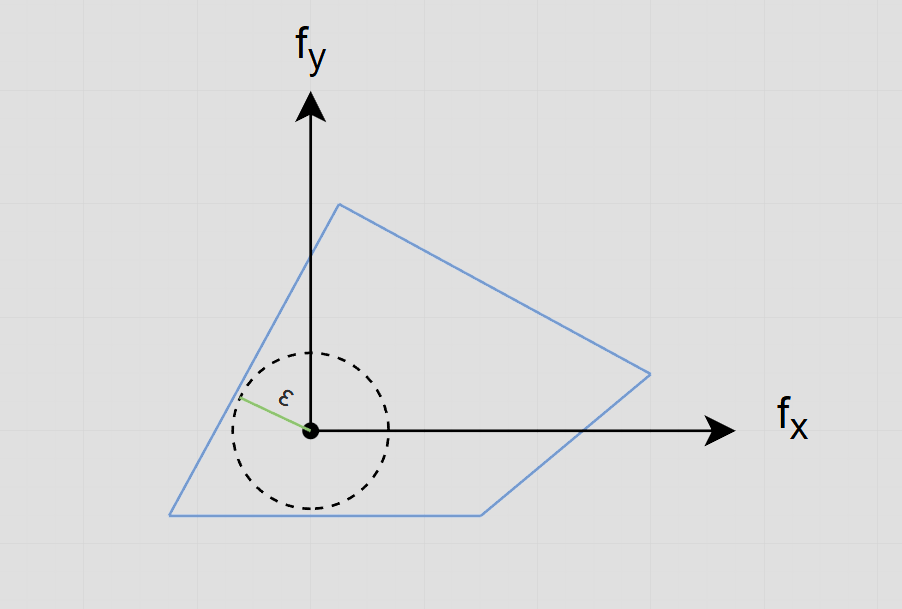
\includegraphics[scale=0.4]{chapter3/image/epsilon.png}
    \caption{Chỉ số Ferrari-Canny $\epsilon$}
    \label{fig:epsilon}
\end{figure}

Chỉ số Ferrari-Canny $\epsilon$ là một thước đo phổ biến để đánh giá chất lượng của một force-closure grasp. Chỉ số này được định nghĩa là bán kính lớn nhất của khối cầu tâm tại gốc tọa độ nằm hoàn toàn bên trong grasp wrench space, hình (\ref{fig:epsilon}) biểu diễn một minh họa trên một mặt phẳng $\tau = \tau_{\text(rand)}$. Về mặt vật lý, $\epsilon$ biểu thị biên độ wrench nhỏ nhất mà grasp có thể sinh ra theo mọi hướng, do đó $\epsilon$ càng lớnthì grasp càng có khả năng chống lại các nhiễu loạn ngoài ý muốn và càng ổn định. Một grasp có $\epsilon = 0$ không thể đạt force closure, trong khi các grasp có $\epsilon > 0$ không chỉ đạt closure mà còn có chất lượng khác nhau tùy theo giá trị $\epsilon$. Chỉ số này vì thế vừa phản ánh khả năng chống nhiễu vừa biểu thị tính “đều” trong phân bố lực mà grasp có thể tạo ra, và nhờ đó được sử dụng rộng rãi trong lập kế hoạch và tối ưu hóa grasp.

\subsection{Bài toán tối ưu tìm lực grasp}
\label{subsec:qp0}
Khi một wrench mong muốn $\mathbf{w}$ nằm trong miền GWS, có thể khẳng định rằng tồn tại một tập các lực $\mathbf{f} = [f_1 \ldots f_k]$ tương ứng tại k điểm tiếp xúc sao cho tổng hợp lực sinh ra wrench mong muốn lên vật thế. Tuy nhiên, câu hỏi tiếp theo là: làm thế nào để tính được các lực tiếp xúc cụ thể này. Một cách đơn giản nhất đó là giải phương trình cân bằng (\ref{eq:wrench2}). Tuy nhiên cách này không hợp lệ trong thực tế vì nó bỏ qua các ràng buộc vật lý quan trọng như là ma sát, giới hạn và chiều có thể tác dụng lực thực tế. Ngoài ra, phương trình có thể có vô số nghiệm, khiến việc lựa chọn bộ lực khả thi trở nên rắc rối hơn.

Do đó, cách tiếp cận phổ biến nhất là giải bài toán tối ưu có ràng buộc tìm lực $\mathbf{f} = [f_1 \ldots f_k]$ sao cho (\ref{eq:wrench2}) được thỏa mãn, với ràng buộc $\mathbf{f}_i \in \mathcal{C}$ với i từ 1 đến k, trong đó $\mathcal{C}$ là tập các ràng buộc lồi (convex constraint set) áp dụng lên lực tiếp xúc $\mathbf{f}_i$ ngoài mô hình nón ma sát. Bài toán có thể được mô hình hóa như sau:
\begin{equation}
\label{eq:forceop}
\begin{aligned}
\min_{f_i,\; i\in\{1,\ldots,k\}} \quad 
    & J(f_1,\ldots,f_k), \\[4pt]
\text{s.t.} \quad 
    & f_i \in \mathcal{F}_i,\quad i=1,\ldots,k, \\[2pt]
    & f_i \in \mathcal{C},\quad i=1,\ldots,k, \\[2pt]
    & w - G 
    \begin{bmatrix}
    f_1 & \dots & f_k
    \end{bmatrix}^T = 0.
\end{aligned}
\end{equation}

trong đó $J$ là hàm mục tiêu lồi theo mỗi $\mathbf{f}_i$, một lựa chọn khá phổ biến là $J(f_1,\ldots,f_k) = \max_i \|f_i\|$ nhằm giảm lực tối đa phải sinh ra tại bất kỳ tiếp điểm nào (giảm quá tải, tăng độ bền hệ thống). 